\documentclass[border=10pt]{standalone}

\usepackage{tikz}
\usepackage{tikzsymbols}
\usetikzlibrary{calc,patterns,shapes.geometric}

\def\centerarc[#1](#2)(#3:#4:#5){\draw[#1] ($(#2)+({#5*cos(#3)},{#5*sin(#3)})$) arc (#3:#4:#5);}

\begin{document}
	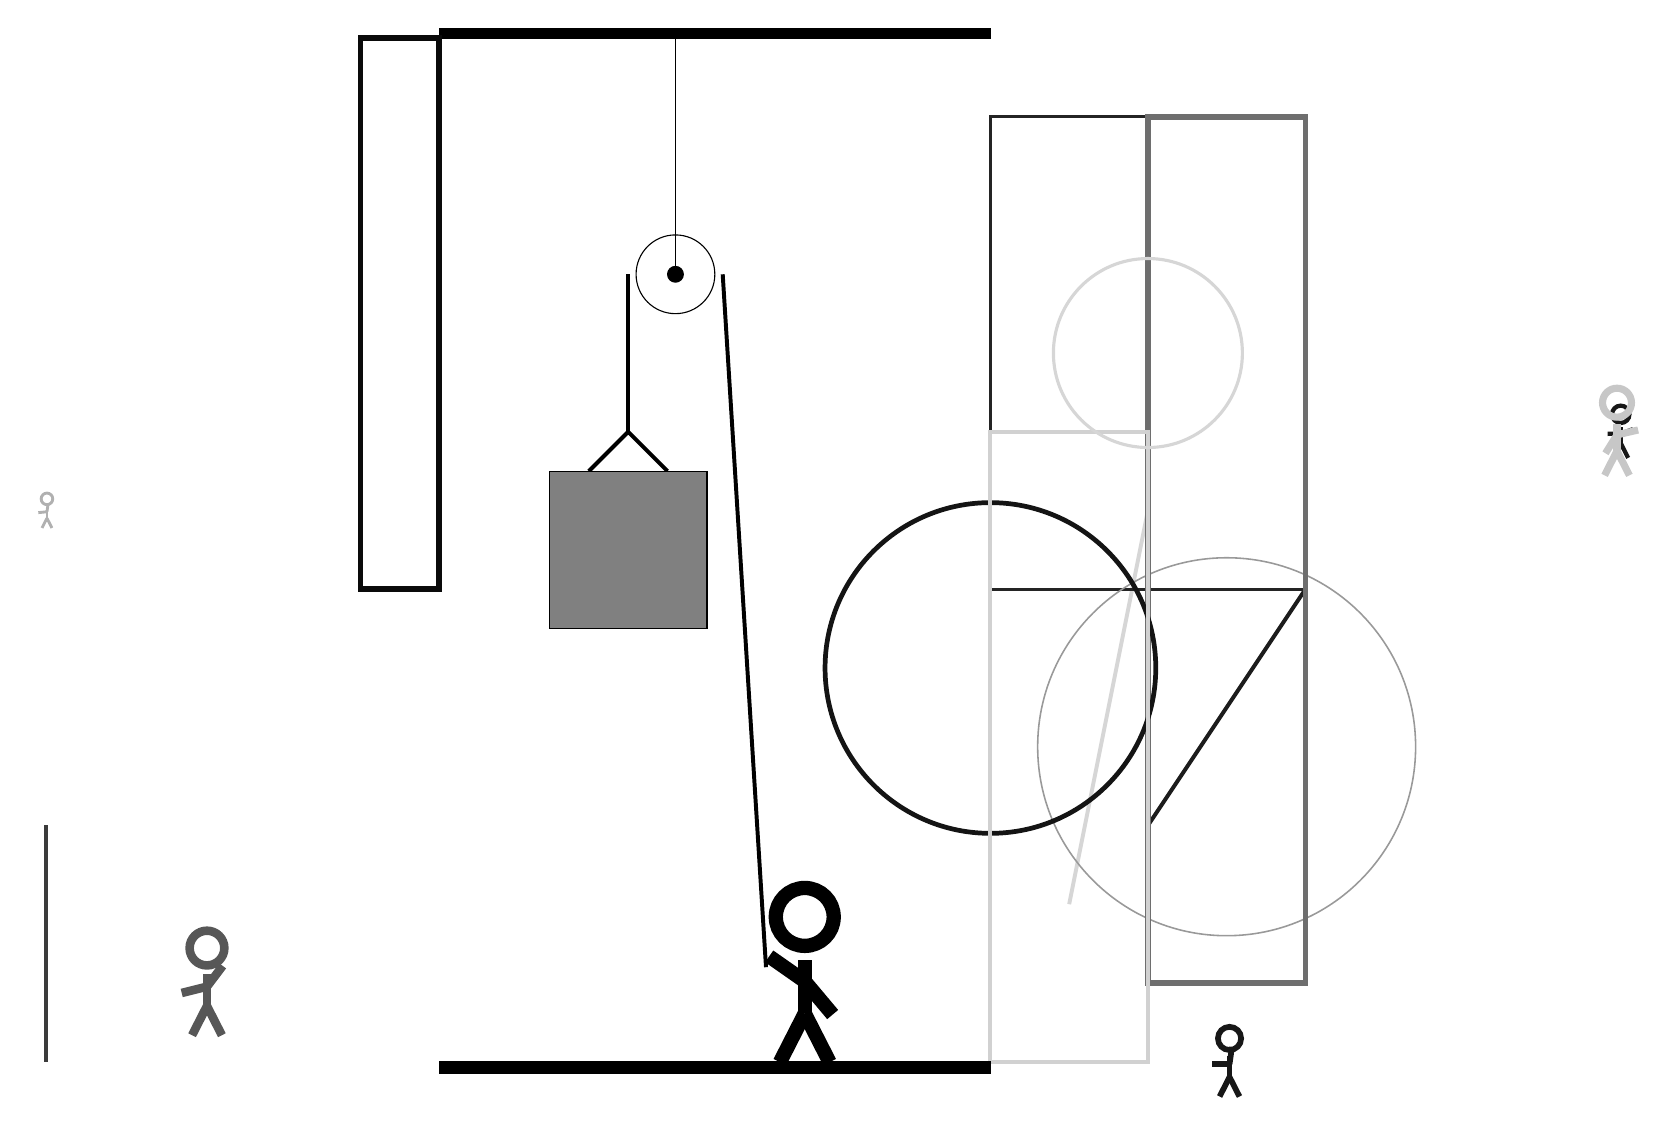
\begin{tikzpicture}
		%%%%% START %%%%%
		
		\draw[fill=black] (-2, 10) rectangle (5, 10.125);
		
		\draw (1, 7) circle (0.5);
		\draw[fill=black] (1, 7) circle (0.1);
		\draw (1, 10) -- (1, 7);
		
		\draw[line width=0.5mm, color=black!16](7, 4) -- (6, -1);
		
		\draw[line width=0.5mm, color=black!89](9, 3) -- (7, 0);
		\draw[line width=0.4mm, color=black!86] (5, 3) rectangle (9, 9);
		\node[line width=0.6mm, color=black!91] at (8, -3) {\Strichmaxerl[4][0][82]};
		
		\draw [line width=0.2mm, color=black!40](8, 1) circle (2.4);
		\draw[line width=0.7mm, color=black!57] (7, 9) rectangle (9, -2);
		\node[line width=0.6mm, color=black!66] at (-5, -2) {\Strichmaxerl[6][14][53]};
		\draw [line width=0.6mm, color=black!92](5, 2) circle (2.1);
		\draw[line width=0.7mm, color=black!96] (-3, 10) rectangle (-2, 3);
		
		\node[line width=0.4mm, color=black!31] at (-7, 4) {\Strichmaxerl[2][6][82]};
		\draw[line width=0.5mm, color=black!18] (7, -3) rectangle (5, 5);
		\node[line width=0.2mm, color=black!91] at (13, 5) {\Strichmaxerl[3][1][20]};
		\draw [line width=0.4mm, color=black!16](7, 6) circle (1.2);
		
		\node[line width=0.3mm, color=black!22] at (13, 5) {\Strichmaxerl[5][58][13]};
		\draw[line width=0.5mm, color=black!77](-7, -3) -- (-7, 0);
		
		\draw[line width=0.5mm] (-0.1, 4.5) -- (0.4, 5.0) -- (0.9, 4.5);
		\draw[fill=black!50] (-0.6, 4.5) rectangle (1.4, 2.5);
		
		\draw[line width=0.5mm] (0.4, 7) -- (0.4, 5.0);
		\centerarc[line width=0.5mm](1, 7)(0:180:0.6);
		\draw[line width=0.5mm](1.6, 7) -- (2.15, -1.8);
		
		\node at (2.6, -1.9) {\Strichmaxerl[10][-35][-50]};
		
		\draw[fill=black] (-2, -3) rectangle (5, -3.15);
		
		%%%%% END %%%%%
	\end{tikzpicture}
\end{document}